% AP-2 Generator Pipeline diagram
% Used in §6.2.3 (ssec:ap2-generator)

\tikzsetnextfilename{ch6-polymul-ap2-pipeline}
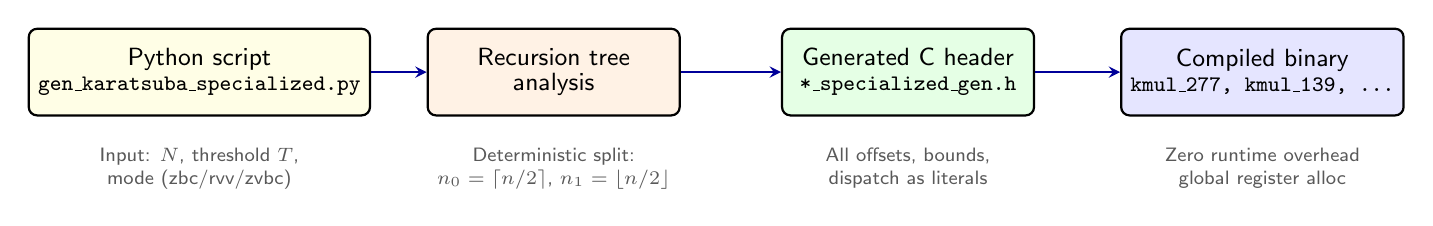
\begin{tikzpicture}[
  stage/.style={draw, rounded corners=3pt, minimum width=3.2cm,
    minimum height=1.1cm, align=center, font=\sffamily\small, thick},
  arrow/.style={->, thick, >=stealth, color=blue!60!black},
  note/.style={font=\sffamily\scriptsize, text=gray!70!black, align=center}
]

% Stage 1: Python script
\node[stage, fill=yellow!10] (script) at (0,0)
  {Python script\\[-2pt]\texttt{\footnotesize gen\_karatsuba\_specialized.py}};

% Stage 2: Recursion tree analysis
\node[stage, fill=orange!10] (tree) at (4.5,0)
  {Recursion tree\\[-2pt]analysis};

% Stage 3: Generated C header
\node[stage, fill=green!10] (header) at (9,0)
  {Generated C header\\[-2pt]\texttt{\footnotesize *\_specialized\_gen.h}};

% Stage 4: Compiled binary
\node[stage, fill=blue!10] (binary) at (13.5,0)
  {Compiled binary\\[-2pt]\texttt{\footnotesize kmul\_277, kmul\_139, \ldots}};

% Arrows
\draw[arrow] (script) -- (tree);
\draw[arrow] (tree) -- (header);
\draw[arrow] (header) -- (binary);

% Annotations below
\node[note, below=8pt] at (script.south) {Input: $N$, threshold $T$,\\mode (zbc/rvv/zvbc)};
\node[note, below=8pt] at (tree.south) {Deterministic split:\\$n_0 = \lceil n/2 \rceil$, $n_1 = \lfloor n/2 \rfloor$};
\node[note, below=8pt] at (header.south) {All offsets, bounds,\\dispatch as literals};
\node[note, below=8pt] at (binary.south) {Zero runtime overhead\\global register alloc};

\end{tikzpicture}
